\chapter{Software Project Telemetry}
\label{Chapter:Telemetry}

Software project telemetry is a novel light-weight software measurement approach. It includes both (1) highly automated measurement machinery for metrics collection and analysis, and (2) a methodology for in-process, empirically-guided software development process problem detection and diagnosis. In this approach, sensors collect software metrics automatically and unobtrusively. Metrics are abstracted to telemetry streams, charts, and reports through a domain-specific language for the representation of telemetry trends for high-level perspectives on software development processes. 
Compared to traditional metrics-based approaches, which are based primarily on historical project databases and model-based comparison, software project telemetry emphasizes project dynamics and in-process control. The comparison in software project telemetry involves much smaller time scales. The idea is that comparison can be made between two different periods of the same project instead of between two different projects, and that the changes in the development process and their trends can be used as the basis for decision-making in project management and process improvement.

This chapter is organized into the following sections. 
Section \ref{Telemetry:Overview} gives an overview of software project telemetry and its essential characteristics.
Section \ref{Telemetry:Data} discusses sensor-based metrics collection. 
Section \ref{Telemetry:Component} discusses telemetry language and telemetry constructs such as stream, chart, and report.
Section \ref{Telemetry:Process} discusses the telemetry-based methodology for 
        project management and process improvement.
Section \ref{Telemetry:Conclusion} summarizes this chapter.





%%%%%%%%%%%%%%%%%%%%%%%%%%%%%%%%%%%%%%%%%%%%%%%%%%%%%%%%%
%                                                       %
%                   S E C T I O N                       %
%                                                       %
%%%%%%%%%%%%%%%%%%%%%%%%%%%%%%%%%%%%%%%%%%%%%%%%%%%%%%%%%

\section{Overview} 
\label{Telemetry:Overview}

Encyclopedia Britannica defines telemetry as ``highly automated communication process by which data are collected from instruments located at remote or inaccessible points and transmitted to receiving equipment for measurement, monitoring, display, and recording.'' Perhaps the highest profile user of telemetry is NASA, where telemetry has been used since 1965 to monitor space flights starting from the early Gemini missions to the modern Mars rovers. Telemetry data, collected by sensors attached to a space vehicle and its occupants, are used for many purposes, such as gaining better insight into mission status, detecting early signals of anomalies, and analyzing impacts of mission adjustments.

The same concept can be applied to software project management: software project telemetry is an automated process and product measurement approach. It is used to gain insight into software development processes, detect early signals of project failures, and analyze impact of project decisions. In this approach, sensors unobtrusively collect time-stamped software metrics, which are abstracted into telemetry streams, charts, and reports. Trends in telemetry streams serve as the basis for project management and process improvement. Telemetry charts and reports provide visualization. By detecting changes and covariance in trends of different metrics, software project telemetry enables a more incremental, visible, and experiential approach to project decision-making. It has the following essential characteristics:

\begin{enumerate}
  \item Software project telemetry data are collected automatically by sensors that unobtrusively monitor some form of state in the project development environment.  In other words, software developers are working in a ``remote or inaccessible location'' from the perspective of metrics collection activities. This contrasts with software metrics data that require human intervention or developer effort to collect, such as PSP/TSP metrics \cite{Humphrey:1995}.
  
  \item Software project telemetry data consist of a stream of time-stamped events, where the time-stamp is significant for analysis. Software project telemetry is thus focused on evolutionary process in software development.  This contrasts, for example, with COCOMO \cite{Cocomo:1981, Cocomo:2000}, where the time at which the calibration data are collected about the project is not significant.
  
  \item Software project telemetry data are continuously updated and immediately available to both developers and managers. Telemetry data are not hidden away in some obscure database guarded by the software quality improvement group. They are easily visible to all members of the project for interpretation. 

  \item Software project telemetry exhibits graceful degradation. While complete sensor data provide best support for project management, telemetry analyses still provide decision-making value even if there is occasional dropout of sensor data, or if data collection starts midway through a project.      
  
  \item Software project telemetry is used for in-process monitoring, control, and short-term prediction. Telemetry analyses provide representations of current project state and how it is changing at various time scales. The simultaneous display of multiple project state values and how they change over the same time periods allow opportunistic analyses --- the emergent knowledge that one state variable appears to co-vary with another in the context of the current project.
  
\end{enumerate}





%%%%%%%%%%%%%%%%%%%%%%%%%%%%%%%%%%%%%%%%%%%%%%%%%%%%%%%%%
%                                                       %
%                   S E C T I O N                       %
%                                                       %
%%%%%%%%%%%%%%%%%%%%%%%%%%%%%%%%%%%%%%%%%%%%%%%%%%%%%%%%%

\section{Sensor-based Data Collection}
\label{Telemetry:Data}

In software project telemetry, metrics are collected \textit{automatically} by sensors that \textit{unobtrusively} monitor some form of state in the project development environment. Sensors are pieces of software collecting both process and product metrics.

Software process metrics are the metrics that assist in monitoring and controlling the way software is produced. Sensors collecting process metrics are typically implemented in the form of plug-ins, which are attached to software development tools in order to continuously monitor and record their activities in the background. Some examples are listed below:

\begin{itemize}

	\item A plug-in for an IDE (integrated development environment) such as Visual Studio \cite{Software:VisualStudio}, and Eclipse \cite{Software:Eclipse}. It can record individual developer activities automatically and transparently, such as code editing effort, compilation attempts, and results, etc.

  \item A plug-in for a version control system, such as Clear Case \cite{Software:ClearCase}, CVS \cite{Software:CVS}, and SVN \cite{Software:SVN}. It can monitor code check-in and check-out activities, and compute \textit{diff} information between different revisions.
  
  \item A plug-in for a bug tracking or issue management system, such as Bugzilla \cite{Software:Bugzilla}, and Jira \cite{Software:Jira}. Whenever an issue is reported or its status is updated, the sensor can detect such activities and record the relevant information.
  
  \item A plug-in for an automated build system, such as Cruise Control \cite{Software:CruiseControl}. It can capture information related to build attempts and build results.

\end{itemize}


Software product metrics are the metrics that describe the properties of the software itself. Sensors collecting product metrics are typically implemented as analyzers for software artifacts. These analyzers usually need to be scheduled to run periodically in order to acquire the continual flow of metrics required by telemetry streams. To automate these tasks, one can use a \textit{Cron} job\footnote{\textit{Cron} is a \textit{Unix/Linux} program that enables users to execute commands or scripts automatically at a specified time or date. The \textit{Windows} equivalent is called \textit{Scheduled Tasks}.}, or run them as tasks in automated build system. Some examples are listed below:

\begin{itemize}

	\item An analyzer that parses program source code to compute size or complexity information.
	
	\item An analyzer that parses the output of existing tools, such as Clover \cite{Software:Clover}, and JBlanket \cite{Software:JBlanket}, and converts them to a data format that can be used by software project telemetry.

\end{itemize}

There are many other possibilities. One can even imagine an exotic sensor that retrieves project cost and payroll information from a company's accounting database, if extraction of such information is permitted by the company policy. The point is: no matter what the sensor does and regardless of its implementation details, a sensor-based approach collects metrics \textit{automatically} and \textit{unobtrusively} in order to keep data collection cost low, so that developers are not distracted from their primary tasks -- developing software products instead of capturing process and product metrics.

This sensor-based approach eliminates the chronic overhead in metrics collection. While setting up sensors might require some effort, once they are installed and configured, sensor data collection is automatic. This contrasts with traditional data collection techniques, such as the paper-and-pencil based approach used in PSP/TSP \cite{Humphrey:1995}, or the tool-supported approach used in LEAP \cite{Moore:1999}, PSP Studio \cite{PspStudio:1997}, and Software Process Dashboard \cite{PspDashboard:2000}. These approaches require constant human intervention or developer effort to collect metrics. Even in the case of the tool-supported approach, the developer still cannot escape the chronic overhead of constantly switching back and forth between doing work and telling the tool what work is being done \cite{Johnson:2001, Johnson:2003}.

The fact that chronic overhead is eliminated from sensor-based metrics collection not only reduces the technology adoption barrier, but also makes it feasible for software organizations to apply measurement to a wide range of development activities and products in order to get a comprehensive quantitative view of development processes.


Admittedly, the sensor-based approach does come with some restrictions:

\begin{itemize}
	
	\item A sensor must be developed for each type of tool we wish to monitor. This is a one-time cost. Once the sensor is developed, it can be used by different software development organizations for different projects. The Collaborative Software Development Lab has already developed a repository of over 25 sensors for commonly-used tools.

  \item Some metrics may not be amenable to automated data collection. An example is software development effort. While it is feasible to instrument an IDE to automatically get information such as how many hours a developer has spent on writing code, it is almost impossible to construct a sensor that knows how much total effort a developer has contributed to a project. For instance, two developers might be discussing the design of a system in the hallway. It is almost impossible to collect this type of effort in an automated way. It is still an open research question whether \textit{all} important metrics can be captured by sensors or not. However, this research takes a more pragmatic view: it is only concerned with whether sensors can collect \textit{sufficient} metrics so that software project telemetry has decision-making value for project management and process improvement. 
 
\end{itemize}






%%%%%%%%%%%%%%%%%%%%%%%%%%%%%%%%%%%%%%%%%%%%%%%%%%%%%%%%%
%                                                       %
%                   S E C T I O N                       %
%                                                       %
%%%%%%%%%%%%%%%%%%%%%%%%%%%%%%%%%%%%%%%%%%%%%%%%%%%%%%%%%

\section{Telemetry Language and Telemetry Constructs} 
\label{Telemetry:Component}

Many interesting issues in software project management involve understanding the relationship between different measures. For example, we might be interested in seeing whether an increased investment in code review pays off with less unit test failures, and/or increased coverage, and/or less defects reported against the reviewed modules. Such questions require comparing a set of metrics values over time. The telemetry language provides a mechanism that facilitates interactive exploration of relationships between metrics.
%so that developers and managers can ``play with the data'' to see what perspectives provide insight to their particular situation.
The language has the following syntax:

\begin{verbatim}
  streams <StreamName> (<ParameterList>) = {
    <DocumentationString>, 
    <Expresion>
  };
    
  y-axis <YAxisName> (<Parameter>) = {
    label, 'integer|double|auto', lowerBound, upperBound
  };
  
  chart  <ChartName>  (<ParameterList>) = {
    <ChartTitile>, 
    <StreamReferences>
  };
    
  report <ReportName> (<ParameterLilst>) = {
    <ReportTitle>, 
    <ChartReferences>
  };
\end{verbatim}


Note, however, that the above syntax is not written in a strict mathematical notation. The formal grammar of the language can be found in Appendix \ref{Chapter:TelemetryLanguageSpecification}: \textit{Software Project Telemetry Language Specification}. 
Chapter \ref{Chapter:Intro} contains a real-world example of the language in Section \ref{Intro:Solution:MetricsAnalysis:TelemetryLanguage}, and the resulting telemetry report in Figure \ref{fig:TelemetryReportChartStream}.


Telemetry \textit{reports}, \textit{charts}, and \textit{streams} are basic constructs of the language. The relationship between them is illustrated in Figure \ref{fig:TelemetryReportChartStream} and discussed in Section \ref{Intro:Solution:MetricsAnalysis}. 
In essence, a telemetry report is a named set of telemetry charts that can be generated for a specified project over a specified time interval. The goal of a telemetry report is to discover how the trajectory of different process and product metrics might influence each other over time, and whether these influences change depending upon context.
A telemetry chart is a named set of telemetry streams. The goal of a telemetry chart is to display the trajectory of one or more process or product metrics over time. The \textit{y-axis} construct is used to specify the vertical axis of a telemetry chart. Note, however, that a telemetry chart definition does not include the information about its horizontal axis, because such information can be automatically inferred from the time interval over which the telemetry analysis is performed. 
A telemetry stream is a sequence of a single type of software process or product metrics. 
%Telemetry streams are best thought of as a kind of abstract data type representing one or more series of metric values of a similar type.
 
The data collected by sensors are time-stamped, and the time stamp is always significant in telemetry style metrics analysis. There may not be a simple one-to-one correspondence between sensor data and the data points in telemetry streams. Sensor data usually represents very fine-grained low level software process or product details, while the data points in telemetry streams represent higher level perspectives on the software system or its development process. Typically, sensor data need to be filtered, combined, and aggregated to derive a telemetry data point. 
For example, suppose we want to construct a telemetry stream representing the number of open bugs for a software project on a monthly interval for the entire year 2005. In addition, suppose we are using Bugzilla \cite{Software:Bugzilla}, and whenever a bug is opened or closed, the Bugzilla sensor records information such as event time stamp, event type (bug open or bug close), bug id, severity, etc. In order to compute the number of open bugs for each month in 2005, the telemetry reducer needs to scan the entire bug event sensor data and combine them in order to compute values for the telemetry data points.  
  
Telemetry reducers takes sensor data as input and output a series of telemetry data points. They are the ``atomic'' building blocks for telemetry constructs at the user level. They serve as the link between sensor data and telemetry streams. They can be thought of as the fixed ``alphabet'' from which any number of telemetry streams can be created by a user. A reducer must be available in order to construct a \textit{``simple''} telemetry stream\footnote{Telemetry streams can also be generated by applying mathematical operations or telemetry functions to existing telemetry streams. These are called \textit{``compound''} telemetry streams as opposed to \textit{``simple''} telemetry streams.}. Some example of general classes of telemetry streams are:

\begin{itemize}
	\item \textbf{Development Telemetry} --- These are telemetry streams generated from data gathered by observing the behavior of software developers as reflected in their tool usage, such as the information about the files they edit, the time they spend using various tools, and the changes they make to project artifacts, the sequences of tool or command invocations, and so forth. Such metrics can be collected by attaching sensors to Integrated Development Environments (e.g., Visual Studio, Eclipse, Emacs), configuration management system (e.g., CVS \cite{Software:CVS}, Clear Case \cite{Software:ClearCase}), issue management systems(e.g., Bugzilla \cite{Software:Bugzilla}, Jira \cite{Software:Jira}), etc.
	
	\item \textbf{Build Telemetry} --- These are telemetry streams generated from data gathered by observing the results of tools invoked to compile, link, and test the system. Such metrics can be collected by attaching sensors to build tools (e.g., Make, Ant \cite{Software:Ant}, Cruise Control \cite{Software:CruiseControl}), testing tools(e.g., JUnit \cite{Software:JUnit}), size and complexity counters(e.g., LOCC \cite{Software:LOCC}), etc.
	
	\item \textbf{Execution Telemetry} --- These are telemetry streams generated from data gathered by observing the behavior of the system as it executes. Such metrics can be collected by sensors attached to the system runtime environment to gather its internal state data (e.g., heap size, occurrence of exceptions), or to load testing tools (e.g., JMeter \cite{Software:JMeter}) of the system to gather system performance data.
	
	\item \textbf{Usage Telemetry} --- These are telemetry streams generated from data gathered by observing the behavior of users as they interact with the system, such as the frequency, types, and sequences of command invocations during a given period of time in a given system.

\end{itemize}











%%%%%%%%%%%%%%%%%%%%%%%%%%%%%%%%%%%%%%%%%%%%%%%%%%%%%%%%%
%                                                       %
%                   S E C T I O N                       %
%                                                       %
%%%%%%%%%%%%%%%%%%%%%%%%%%%%%%%%%%%%%%%%%%%%%%%%%%%%%%%%%

\section{Telemetry-guided Project Management and Process Improvement} 
\label{Telemetry:Process}

The basic steps of telemetry-guided process improvement are illustrated in Figure \ref{fig:TelemetryBasedProcessImprovement}. It involves cycles of problem detection, process improvement hypothesis generation, process change implementation, hypothesis validation, and impact analysis.
Following Hetzel \cite{Hetzel:1993}, a software organization is recommended to collect a basic set of metrics, such as code size, test coverage, and build results, for every project at all time. This basic set of metrics generates a basic set of telemetry streams, which provide insights into the current software development practice and help establish a base line for the current process.

\begin{figure}[p]
  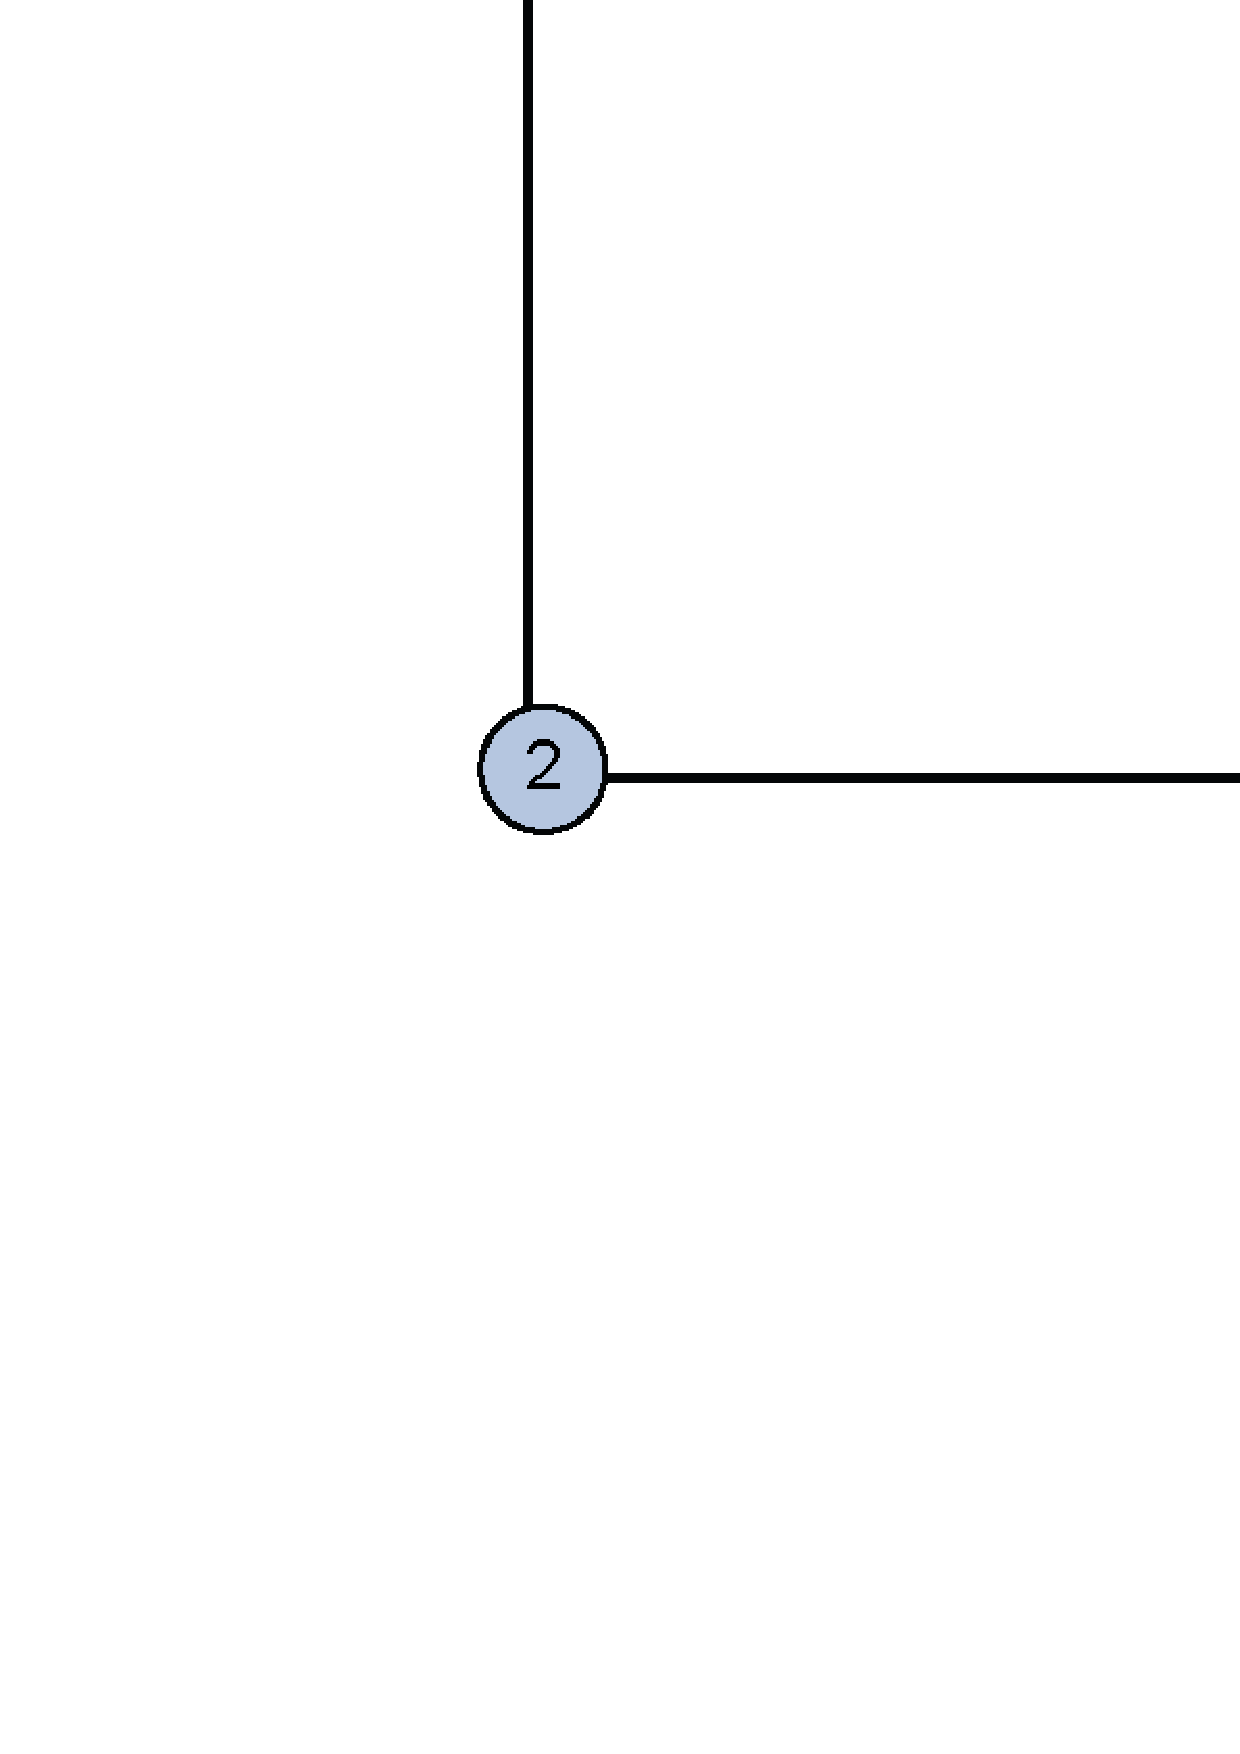
\includegraphics[width=1.00\textwidth]{figures/TelemetryProcess}
  \caption{Telemetry-based Process Improvement} 
  \label{fig:TelemetryBasedProcessImprovement}
\end{figure}


Software project telemetry can be used in two modes: (1) \textit{in-process project monitoring}, and (2) \textit{process improvement}. The two modes are closely related, and sometimes indistinguishable in practice. However, I will keep them separated in this discussion in order to make the concept clear. 

The steps for in-process project monitoring start from the upper arrow in Figure \ref{fig:TelemetryBasedProcessImprovement}. Telemetry streams are monitored for anomalies and unfavorable trends. If anomalies or unfavorable trends are detected, then the project manager must investigate the cause. Multiple telemetry streams, representing different perspectives on the development process, can be used to detect correlations. For example, the project manager might find that complexity telemetry values are increasing as well as defect density. Since telemetry streams consist of time-stamped events, the sequence of detected changes might help the project manager generate hypothesis about the causal relationship and corrective measures for process improvement. For example, the project manager might identify code complexity as a likely cause for high defect density. Once the process improvement hypothesis is generated, the project manager tries corrective actions such as simplifying over-complex modules, and continues to monitor telemetry streams in order to check whether the action results in a decrease in defect density. The project manager can also monitor other telemetry streams to check if such corrective action has unintended side-effects (impact analysis). If the hypothesis is correct, it will be validated by the newly-generated telemetry streams. If the telemetry streams indicate otherwise, then there must be other reasons that cause high defect density, and the project manager must try other corrective measures.

The steps for process improvement follow the same loop as the steps for in-process project monitoring. The only difference is that they start from the lower arrow in Figure \ref{fig:TelemetryBasedProcessImprovement}, and implementation of process improvement measures does  not have to wait until anomalies or unfavorable trends are detected in telemetry streams. 








%%%%%%%%%%%%%%%%%%%%%%%%%%%%%%%%%%%%%%%%%%%%%%%%%%%%%%%%%
%                                                       %
%                   S E C T I O N                       %
%                                                       %
%%%%%%%%%%%%%%%%%%%%%%%%%%%%%%%%%%%%%%%%%%%%%%%%%%%%%%%%%

\section{Chapter Summary}
\label{Telemetry:Conclusion}

In this chapter, I have described Software Project Telemetry in theory. It includes both (1) highly automated measurement machinery for metrics collection and analysis, and (2) a methodology for in-process, empirically-guided software development process problem detection and diagnosis. The next chapter introduces the tool implementation.

